% Options for packages loaded elsewhere
\PassOptionsToPackage{unicode}{hyperref}
\PassOptionsToPackage{hyphens}{url}
%
\documentclass[
]{article}
\usepackage{amsmath,amssymb}
\usepackage{iftex}
\ifPDFTeX
  \usepackage[T1]{fontenc}
  \usepackage[utf8]{inputenc}
  \usepackage{textcomp} % provide euro and other symbols
\else % if luatex or xetex
  \usepackage{unicode-math} % this also loads fontspec
  \defaultfontfeatures{Scale=MatchLowercase}
  \defaultfontfeatures[\rmfamily]{Ligatures=TeX,Scale=1}
\fi
\usepackage{lmodern}
\ifPDFTeX\else
  % xetex/luatex font selection
\fi
% Use upquote if available, for straight quotes in verbatim environments
\IfFileExists{upquote.sty}{\usepackage{upquote}}{}
\IfFileExists{microtype.sty}{% use microtype if available
  \usepackage[]{microtype}
  \UseMicrotypeSet[protrusion]{basicmath} % disable protrusion for tt fonts
}{}
\makeatletter
\@ifundefined{KOMAClassName}{% if non-KOMA class
  \IfFileExists{parskip.sty}{%
    \usepackage{parskip}
  }{% else
    \setlength{\parindent}{0pt}
    \setlength{\parskip}{6pt plus 2pt minus 1pt}}
}{% if KOMA class
  \KOMAoptions{parskip=half}}
\makeatother
\usepackage{xcolor}
\usepackage[margin=1in]{geometry}
\usepackage{color}
\usepackage{fancyvrb}
\newcommand{\VerbBar}{|}
\newcommand{\VERB}{\Verb[commandchars=\\\{\}]}
\DefineVerbatimEnvironment{Highlighting}{Verbatim}{commandchars=\\\{\}}
% Add ',fontsize=\small' for more characters per line
\usepackage{framed}
\definecolor{shadecolor}{RGB}{248,248,248}
\newenvironment{Shaded}{\begin{snugshade}}{\end{snugshade}}
\newcommand{\AlertTok}[1]{\textcolor[rgb]{0.94,0.16,0.16}{#1}}
\newcommand{\AnnotationTok}[1]{\textcolor[rgb]{0.56,0.35,0.01}{\textbf{\textit{#1}}}}
\newcommand{\AttributeTok}[1]{\textcolor[rgb]{0.13,0.29,0.53}{#1}}
\newcommand{\BaseNTok}[1]{\textcolor[rgb]{0.00,0.00,0.81}{#1}}
\newcommand{\BuiltInTok}[1]{#1}
\newcommand{\CharTok}[1]{\textcolor[rgb]{0.31,0.60,0.02}{#1}}
\newcommand{\CommentTok}[1]{\textcolor[rgb]{0.56,0.35,0.01}{\textit{#1}}}
\newcommand{\CommentVarTok}[1]{\textcolor[rgb]{0.56,0.35,0.01}{\textbf{\textit{#1}}}}
\newcommand{\ConstantTok}[1]{\textcolor[rgb]{0.56,0.35,0.01}{#1}}
\newcommand{\ControlFlowTok}[1]{\textcolor[rgb]{0.13,0.29,0.53}{\textbf{#1}}}
\newcommand{\DataTypeTok}[1]{\textcolor[rgb]{0.13,0.29,0.53}{#1}}
\newcommand{\DecValTok}[1]{\textcolor[rgb]{0.00,0.00,0.81}{#1}}
\newcommand{\DocumentationTok}[1]{\textcolor[rgb]{0.56,0.35,0.01}{\textbf{\textit{#1}}}}
\newcommand{\ErrorTok}[1]{\textcolor[rgb]{0.64,0.00,0.00}{\textbf{#1}}}
\newcommand{\ExtensionTok}[1]{#1}
\newcommand{\FloatTok}[1]{\textcolor[rgb]{0.00,0.00,0.81}{#1}}
\newcommand{\FunctionTok}[1]{\textcolor[rgb]{0.13,0.29,0.53}{\textbf{#1}}}
\newcommand{\ImportTok}[1]{#1}
\newcommand{\InformationTok}[1]{\textcolor[rgb]{0.56,0.35,0.01}{\textbf{\textit{#1}}}}
\newcommand{\KeywordTok}[1]{\textcolor[rgb]{0.13,0.29,0.53}{\textbf{#1}}}
\newcommand{\NormalTok}[1]{#1}
\newcommand{\OperatorTok}[1]{\textcolor[rgb]{0.81,0.36,0.00}{\textbf{#1}}}
\newcommand{\OtherTok}[1]{\textcolor[rgb]{0.56,0.35,0.01}{#1}}
\newcommand{\PreprocessorTok}[1]{\textcolor[rgb]{0.56,0.35,0.01}{\textit{#1}}}
\newcommand{\RegionMarkerTok}[1]{#1}
\newcommand{\SpecialCharTok}[1]{\textcolor[rgb]{0.81,0.36,0.00}{\textbf{#1}}}
\newcommand{\SpecialStringTok}[1]{\textcolor[rgb]{0.31,0.60,0.02}{#1}}
\newcommand{\StringTok}[1]{\textcolor[rgb]{0.31,0.60,0.02}{#1}}
\newcommand{\VariableTok}[1]{\textcolor[rgb]{0.00,0.00,0.00}{#1}}
\newcommand{\VerbatimStringTok}[1]{\textcolor[rgb]{0.31,0.60,0.02}{#1}}
\newcommand{\WarningTok}[1]{\textcolor[rgb]{0.56,0.35,0.01}{\textbf{\textit{#1}}}}
\usepackage{graphicx}
\makeatletter
\def\maxwidth{\ifdim\Gin@nat@width>\linewidth\linewidth\else\Gin@nat@width\fi}
\def\maxheight{\ifdim\Gin@nat@height>\textheight\textheight\else\Gin@nat@height\fi}
\makeatother
% Scale images if necessary, so that they will not overflow the page
% margins by default, and it is still possible to overwrite the defaults
% using explicit options in \includegraphics[width, height, ...]{}
\setkeys{Gin}{width=\maxwidth,height=\maxheight,keepaspectratio}
% Set default figure placement to htbp
\makeatletter
\def\fps@figure{htbp}
\makeatother
\setlength{\emergencystretch}{3em} % prevent overfull lines
\providecommand{\tightlist}{%
  \setlength{\itemsep}{0pt}\setlength{\parskip}{0pt}}
\setcounter{secnumdepth}{-\maxdimen} % remove section numbering
\ifLuaTeX
  \usepackage{selnolig}  % disable illegal ligatures
\fi
\usepackage{bookmark}
\IfFileExists{xurl.sty}{\usepackage{xurl}}{} % add URL line breaks if available
\urlstyle{same}
\hypersetup{
  pdftitle={HW4},
  pdfauthor={Samuel Olson},
  hidelinks,
  pdfcreator={LaTeX via pandoc}}

\title{HW4}
\author{Samuel Olson}
\date{}

\begin{document}
\maketitle

\section{Outline}\label{outline}

\begin{itemize}
\tightlist
\item
  Q1: g2g
\item
  Q2: e), f), g) left
\item
  Q3: g2g
\item
  Q4: g2g
\end{itemize}

\section{Problem 1}\label{problem-1}

Suppose
\(\boldsymbol{y} = \boldsymbol{X\beta} + \boldsymbol{\varepsilon}\),
where
\(\boldsymbol{\varepsilon} \sim \mathcal{N}(\boldsymbol{0},\sigma^2 \boldsymbol{I})\)
for some unknown \(\sigma^2 > 0\). Let
\(\boldsymbol{\hat{y}} = \boldsymbol{P_X y}\).

\subsection{a)}\label{a}

Determine the distribution of

\[
\begin{bmatrix}
\boldsymbol{\hat{y}} \\ 
\boldsymbol{y - \hat{y}} \\ 
\end{bmatrix}
\]

\subsubsection{Useful Property:}\label{useful-property}

Linear transformation of a normal random variable is itself normal
(distribution remains normal with known/calculable parameters):

\[
\boldsymbol{x} \sim \mathcal{N}(\boldsymbol{\mu}, \boldsymbol{\Sigma}) \rightarrow \boldsymbol{Ax} + \boldsymbol{b} \sim \mathcal{N}(\boldsymbol{A \mu} + \boldsymbol{b}, \boldsymbol{A \Sigma A ^{\top}})
\]

To begin, note the {[}Useful Property{]} provides us reason to assert
that the following follows an MVN distribution:

\[
\begin{bmatrix}
\boldsymbol{\hat{y}} \\ 
\boldsymbol{y - \hat{y}} \\ 
\end{bmatrix}
\sim \mathcal{N}(?, ??)
\]

Such that we need to identify the mean and covariance matrix of the
above.

To that end, note that by definition:

\[
\begin{bmatrix}
\boldsymbol{\hat{y}} \\ 
\boldsymbol{y - \hat{y}} \\ 
\end{bmatrix}
= 
\begin{bmatrix}
\boldsymbol{P_{X}y} \\ 
\boldsymbol{y} - \boldsymbol{P_{X}y} \\ 
\end{bmatrix}
= 
\begin{bmatrix}
\boldsymbol{P_{X}} \\ 
\boldsymbol{I} - \boldsymbol{P_{X}} \\ 
\end{bmatrix} \boldsymbol{y}
\]

To calculate the mean, noting linearity of expectation:

\[
E \left( \begin{bmatrix} \boldsymbol{P_X} \\ \boldsymbol{I} - \boldsymbol{P_X} \end{bmatrix} y \right)
= \begin{bmatrix} \boldsymbol{P_X} \\ \boldsymbol{I} - \boldsymbol{P_X} \end{bmatrix} E(y)
= \begin{bmatrix} \boldsymbol{P_X} \\ \boldsymbol{I} - \boldsymbol{P_X} \end{bmatrix} \boldsymbol{X} \boldsymbol{\beta}
= \begin{bmatrix} \boldsymbol{X} \boldsymbol{\beta} \\ \boldsymbol{X} \boldsymbol{\beta} - \boldsymbol{X} \boldsymbol{\beta} \end{bmatrix}
= \begin{bmatrix} \boldsymbol{X} \boldsymbol{\beta} \\ \boldsymbol{0} \end{bmatrix}
\]

To calculate the covariance, noting properties of the Projection Matrix
(symmetric and idempotent):

\[
\text{Var} \left( 
\begin{bmatrix} 
\boldsymbol{P_X} \\ \boldsymbol{I} - \boldsymbol{P_X} 
\end{bmatrix} 
y \right)
= 
\begin{bmatrix} 
\boldsymbol{P_X} \\ \boldsymbol{I} - \boldsymbol{P_X} 
\end{bmatrix} 
\text{Var}(y) 
\begin{bmatrix} 
\boldsymbol{P_X} \\ \boldsymbol{I} - \boldsymbol{P_X} 
\end{bmatrix}^{\top}
= 
\begin{bmatrix} 
\boldsymbol{P_X} \\ \boldsymbol{I} - \boldsymbol{P_X} 
\end{bmatrix} 
\sigma^2 \boldsymbol{I} 
\begin{bmatrix} 
\boldsymbol{P_X}, (\boldsymbol{I} - \boldsymbol{P_X})^{\top} 
\end{bmatrix}
= \sigma^2 
\begin{bmatrix} 
\boldsymbol{P_X} \boldsymbol{P_X}^{\top} & \boldsymbol{P_X} (\boldsymbol{I} - \boldsymbol{P_X})^{\top} \\ 
(\boldsymbol{I} - \boldsymbol{P_X}) \boldsymbol{P_X}^{\top} & (\boldsymbol{I} - \boldsymbol{P_X}) (\boldsymbol{I} - \boldsymbol{P_X})^{\top} \end{bmatrix}
= \sigma^2 
\begin{bmatrix} \boldsymbol{P_X} & \boldsymbol{P_X} - \boldsymbol{P_X} \\ 
\boldsymbol{P_X} - \boldsymbol{P_X} & \boldsymbol{I} - \boldsymbol{P_X} - \boldsymbol{P_X} + \boldsymbol{P_X} 
\end{bmatrix}
\]

\[
\text{Var} \left( 
\begin{bmatrix} 
\boldsymbol{P_X} \\ \boldsymbol{I} - \boldsymbol{P_X} 
\end{bmatrix} 
y \right) 
= \sigma^2 
\begin{bmatrix} 
\boldsymbol{P_X} & \boldsymbol{0} \\ \boldsymbol{0} & \boldsymbol{I} - \boldsymbol{P_X} 
\end{bmatrix}
\]

Taken together, and again with note of the {[}Useful Property{]}, we
know:

\[
\begin{bmatrix}
\boldsymbol{\hat{y}} \\ 
\boldsymbol{y - \hat{y}} \\ 
\end{bmatrix}
\sim
\mathcal{N} \left( 
\begin{bmatrix} \boldsymbol{X} \boldsymbol{\beta} \\ \boldsymbol{0} \end{bmatrix}, 
\sigma^2 
\begin{bmatrix} 
\boldsymbol{P_X} & \boldsymbol{0} \\ \boldsymbol{0} & \boldsymbol{I} - \boldsymbol{P_X} 
\end{bmatrix}
\right)
\]

\newpage

\subsection{b)}\label{b}

Determine the distribution of

\[
\hat{y}^{\top} \hat{y}
\]

Noting again the properties of the Projection Matrix (symmetric and
idempotent):

\[
\hat{y}^{\top} \hat{y} = [\boldsymbol{P_X} y]^{\top} \boldsymbol{P_X} y = y^{\top} \boldsymbol{P_X}^{\top} \boldsymbol{P_X} y = y^{\top} \boldsymbol{P_X} \boldsymbol{P_X} y
= y^{\top} \boldsymbol{P_X} y
\]

where
\(y \sim \mathcal{N}(\boldsymbol{X} \boldsymbol{\beta}, \sigma^2 \boldsymbol{I})\).

\begin{figure}
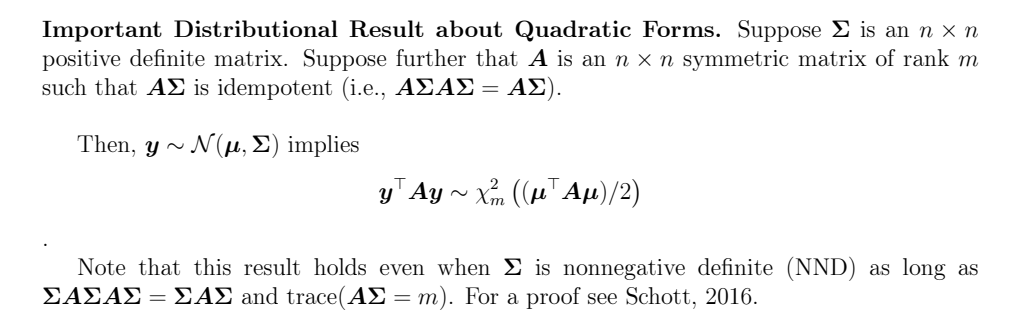
\includegraphics[width=14.39in]{Form} \caption{CocoMelon}\label{fig:unnamed-chunk-3}
\end{figure}

Note the above ``Distributional Result About Quadratic Forms''. This
will be our guide here.

We want to find a matrix \(\boldsymbol{A}\) such that
\(\boldsymbol{A} \boldsymbol{\Sigma}\) is idempotent for
\(\boldsymbol{\Sigma} \equiv \text{Var}(y)\).

One candidate we consider:
\(\boldsymbol{A} = \frac{\boldsymbol{P_X}}{\sigma^2}\)

We first know that this matrix will need to be symmetric. To that end
note:

\[
\boldsymbol{A}^{\top} = \left( \frac{\boldsymbol{P_X}}{\sigma^2} \right) ^ {\top} = \frac{1}{\sigma^2} \left(\boldsymbol{P_X} \right)^{\top} = \frac{1}{\sigma^2} \boldsymbol{P_X} = \boldsymbol{A}
\]

So this matrix is symmetric (because we utilize the Projection Matrix
and multiply it by \(\frac{1}{\sigma^2}\), which preserves symmetry).

Then consider, using the symmetry property shown:

\[
\boldsymbol{A} \boldsymbol{\Sigma} = \boldsymbol{A} \text{Var}(y) = \frac{\boldsymbol{P_X}}{\sigma^2} \sigma^2 \boldsymbol{I} = \boldsymbol{P_X}
\]

So, we then know that
\(\boldsymbol{A}\boldsymbol{\Sigma}  = \boldsymbol{P_X}\) is idempotent,
as the Projection Matrix is idempotent by definition.

We then note: \(\boldsymbol{\Sigma} = \sigma^2 \boldsymbol{I}\) is
positive definite since \(\sigma^2 > 0\).

We use this property to determine the rank of \(\boldsymbol{A}\), with
the goal of determining if it is full rank:

Using the expressions given above:

\[
\text{rank}(\boldsymbol{A}) = \text{rank}(\frac{\boldsymbol{P_X}}{\sigma^2}) = \text{rank}(\boldsymbol{P_X}) = \text{rank}(\boldsymbol{X})
\]

Noting that scalar multiplication (non-zero) does not affect rank
calculations of a matrix.

Then, noting that both \(\hat{y}^{\top}\) and \(\hat{y}\) are normally
distributed, we then know that the quadratic form
\(\hat{y}^{\top} \hat{y}\) is \(\chi^2\) distributed, and that
\(\frac{1}{\sigma^2} \hat{y}^{\top} \hat{y}\) is a scaled \(\chi^2\)
distributed. The degrees of freedom parameter to this distribution is
given by the rank, shown above, and we again make use of
``Distributional Result About Quadratic Forms'' regarding the centrality
parameter.

Taken together, this gives us the expression:

\[
\frac{1}{\sigma^2} \hat{y}^{\top} \hat{y} = y^{\top} \frac{\boldsymbol{P_X}}{\sigma^2} y \sim \chi^2_{\text{rank}(\boldsymbol{X})} \left( \frac{\boldsymbol{X}^{\top} \boldsymbol{A} \boldsymbol{X} \boldsymbol{\beta}}{2} \right)
= \chi^2_{\text{rank}(\boldsymbol{X})} \left( \frac{\boldsymbol{X}^{\top} \frac{\boldsymbol{P_X}}{\sigma^2} \boldsymbol{X} \boldsymbol{\beta}}{2} \right)
= 
\chi^2_{\text{rank}(\boldsymbol{X})} \left( \frac{\boldsymbol{X}^{\top} \boldsymbol{P_X} \boldsymbol{X} \boldsymbol{\beta}}{2 \sigma^2} \right)
\]

Noting the results of the quadratic form:

\[
\mathbf{y} \sim \mathcal{N}(\boldsymbol{\mu}, \boldsymbol{\Sigma})
\rightarrow
\mathbf{y}^{\top} \boldsymbol{A} \mathbf{y} \sim \chi^2_m \left( \frac{\boldsymbol{\mu}^{\top} \boldsymbol{A} \boldsymbol{\mu}}{2} \right)
\]

The remaining point to detail then is the non-centrality parameter.
Knowing the underlying distributions of \(\hat{y}^{\top}\) and
\(\hat{y}\), we then know:

\[
\frac{\boldsymbol{X}^{\top} \boldsymbol{A} \boldsymbol{X} \boldsymbol{\beta}}{2} = \frac{1}{2}\boldsymbol{X}^{\top} \frac{\boldsymbol{P_X}}{\sigma^2} \boldsymbol{X} \boldsymbol{\beta}
= \frac{1}{2 \sigma^2} \boldsymbol{\beta}^{\top} \boldsymbol{X}^{\top} \boldsymbol{P_X} \boldsymbol{X} \boldsymbol{\beta}
= \frac{1}{2 \sigma^2} \boldsymbol{\beta}^{\top} \boldsymbol{X}^{\top} \boldsymbol{X} \boldsymbol{\beta}
\]

Taken together, we then conclude with:

\[
\hat{y}^{\top} \hat{y} \sim \sigma^2 \chi^2_{\text{rank}(\boldsymbol{X})} \left( \frac{\boldsymbol{\beta}^{\top} \boldsymbol{X}^{\top} \boldsymbol{X} \boldsymbol{\beta}}{2\sigma^2} \right)
\]

\newpage

\section{Problem 2}\label{problem-2}

An experiment was conducted to study the durability of coated fabric
subjected to abrasive tests. Three factors were considered:
\textbf{Filler type} with two levels (F1 and F2), \textbf{Surface
treatment} with two levels (S1 and S2), \textbf{Proportion of filler}
with three levels (25\%, 50\%, and 75\%).

Using a completely randomized design with two fabric samples per
treatment, the amount of fabric lost (in mg) for each fabric sample was
recorded. Data are available in a tab-delimited text file at:\\
\href{http://dnett.github.io/S510/FabricLoss.txt}{FabricLoss.txt}.

\begin{Shaded}
\begin{Highlighting}[]
\NormalTok{FabricLoss}\OtherTok{\textless{}{-}} \FunctionTok{read.table}\NormalTok{(}\AttributeTok{file =} \StringTok{"FabricLoss.txt"}\NormalTok{, }
                     \AttributeTok{header =} \ConstantTok{TRUE}\NormalTok{, }
                     \AttributeTok{sep =} \StringTok{"}\SpecialCharTok{\textbackslash{}t}\StringTok{"}\NormalTok{)}
\end{Highlighting}
\end{Shaded}

\begin{Shaded}
\begin{Highlighting}[]
\NormalTok{FabricLoss}\SpecialCharTok{$}\NormalTok{surface }\OtherTok{\textless{}{-}} \FunctionTok{factor}\NormalTok{(FabricLoss}\SpecialCharTok{$}\NormalTok{surface)  }
\NormalTok{FabricLoss}\SpecialCharTok{$}\NormalTok{filler }\OtherTok{\textless{}{-}} \FunctionTok{factor}\NormalTok{(FabricLoss}\SpecialCharTok{$}\NormalTok{filler)}
\NormalTok{FabricLoss}\SpecialCharTok{$}\NormalTok{p }\OtherTok{\textless{}{-}} \FunctionTok{factor}\NormalTok{(FabricLoss}\SpecialCharTok{$}\NormalTok{p)}
\NormalTok{FabricLoss }\OtherTok{\textless{}{-}}\NormalTok{ FabricLoss[}\FunctionTok{order}\NormalTok{(FabricLoss}\SpecialCharTok{$}\NormalTok{surface, FabricLoss}\SpecialCharTok{$}\NormalTok{filler, FabricLoss}\SpecialCharTok{$}\NormalTok{p),]  }

\NormalTok{model }\OtherTok{\textless{}{-}} \FunctionTok{lm}\NormalTok{(y }\SpecialCharTok{\textasciitilde{}} \DecValTok{0} \SpecialCharTok{+}\NormalTok{ surface}\SpecialCharTok{:}\NormalTok{filler}\SpecialCharTok{:}\NormalTok{p, }\AttributeTok{data =}\NormalTok{ FabricLoss)}
\FunctionTok{coef}\NormalTok{(model)}
\end{Highlighting}
\end{Shaded}

\begin{verbatim}
## surface1:filler1:p25 surface2:filler1:p25 surface1:filler2:p25 
##                201.0                164.0                213.0 
## surface2:filler2:p25 surface1:filler1:p50 surface2:filler1:p50 
##                148.5                237.0                187.5 
## surface1:filler2:p50 surface2:filler2:p50 surface1:filler1:p75 
##                233.5                113.5                267.0 
## surface2:filler1:p75 surface1:filler2:p75 surface2:filler2:p75 
##                232.0                234.5                143.5
\end{verbatim}

\begin{Shaded}
\begin{Highlighting}[]
\NormalTok{estimate }\OtherTok{\textless{}{-}} \ControlFlowTok{function}\NormalTok{(lmout, C, }\AttributeTok{a=}\FloatTok{0.05}\NormalTok{)\{}
\NormalTok{  b}\OtherTok{=}\FunctionTok{coef}\NormalTok{(lmout)}
\NormalTok{  V}\OtherTok{=}\FunctionTok{vcov}\NormalTok{(lmout)}
\NormalTok{  df}\OtherTok{=}\NormalTok{lmout}\SpecialCharTok{$}\NormalTok{df}
\NormalTok{  Cb}\OtherTok{=}\NormalTok{C}\SpecialCharTok{\%*\%}\NormalTok{b}
\NormalTok{  se}\OtherTok{=}\FunctionTok{sqrt}\NormalTok{(}\FunctionTok{diag}\NormalTok{(C}\SpecialCharTok{\%*\%}\NormalTok{V}\SpecialCharTok{\%*\%}\FunctionTok{t}\NormalTok{(C)))}
\NormalTok{  tval}\OtherTok{=}\FunctionTok{qt}\NormalTok{(}\DecValTok{1}\SpecialCharTok{{-}}\NormalTok{a}\SpecialCharTok{/}\DecValTok{2}\NormalTok{,df)}
\NormalTok{  low}\OtherTok{=}\NormalTok{Cb}\SpecialCharTok{{-}}\NormalTok{tval}\SpecialCharTok{*}\NormalTok{se}
\NormalTok{  up}\OtherTok{=}\NormalTok{Cb}\SpecialCharTok{+}\NormalTok{tval}\SpecialCharTok{*}\NormalTok{se}
\NormalTok{  m}\OtherTok{=}\FunctionTok{cbind}\NormalTok{(C,Cb,se,low,up)}
  \FunctionTok{dimnames}\NormalTok{(m)[[}\DecValTok{2}\NormalTok{]]}\OtherTok{=}\FunctionTok{c}\NormalTok{(}\FunctionTok{paste}\NormalTok{(}\StringTok{"c"}\NormalTok{,}\DecValTok{1}\SpecialCharTok{:}\FunctionTok{ncol}\NormalTok{(C),}\AttributeTok{sep=}\StringTok{""}\NormalTok{),}
             \StringTok{"estimate"}\NormalTok{,}\StringTok{"se"}\NormalTok{,}
             \FunctionTok{paste}\NormalTok{(}\DecValTok{100}\SpecialCharTok{*}\NormalTok{(}\DecValTok{1}\SpecialCharTok{{-}}\NormalTok{a),}\StringTok{"\% Conf."}\NormalTok{,}\AttributeTok{sep=}\StringTok{""}\NormalTok{),}
             \StringTok{"limits"}\NormalTok{)}
  \FunctionTok{return}\NormalTok{(m)}
\NormalTok{\}}
\end{Highlighting}
\end{Shaded}

Cell Means Model \(\beta\) Matrix:

\[
\boldsymbol{\beta} 
= 
\begin{bmatrix}
\beta_{surface1:filler1:p25} \\ 
\beta_{surface2:filler1:p25} \\
\beta_{surface1:filler2:p25} \\
\beta_{surface2:filler2:p25} \\
\beta_{surface1:filler1:p50} \\
\beta_{surface2:filler1:p50}\\
\beta_{surface1:filler2:p50} \\
\beta_{surface2:filler2:p50} \\
\beta_{surface1:filler1:p75} \\
\beta_{surface2:filler1:p75} \\
\beta_{surface1:filler2:p75} \\
\beta_{surface2:filler2:p75} \\
\end{bmatrix}
\]

\subsection{a)}\label{a-1}

Consider a cell means model for these data. Estimate the mean and
standard error for the treatment corresponding to F2, S1, and 50\%
filler.

\begin{Shaded}
\begin{Highlighting}[]
\CommentTok{\# surface1:filler2:p50}
\NormalTok{C }\OtherTok{=} \FunctionTok{matrix}\NormalTok{(}\FunctionTok{c}\NormalTok{(}\DecValTok{0}\NormalTok{, }\DecValTok{0}\NormalTok{, }\DecValTok{0}\NormalTok{, }\DecValTok{0}\NormalTok{, }\DecValTok{0}\NormalTok{, }\DecValTok{0}\NormalTok{, }
             \DecValTok{1}\NormalTok{, }\DecValTok{0}\NormalTok{, }\DecValTok{0}\NormalTok{, }\DecValTok{0}\NormalTok{, }\DecValTok{0}\NormalTok{, }\DecValTok{0}\NormalTok{),}\AttributeTok{nrow =}\DecValTok{1}\NormalTok{)}

\FunctionTok{estimate}\NormalTok{(}\AttributeTok{lmout =}\NormalTok{ model, }\AttributeTok{C =}\NormalTok{ C)}
\end{Highlighting}
\end{Shaded}

\begin{verbatim}
##      c1 c2 c3 c4 c5 c6 c7 c8 c9 c10 c11 c12 estimate       se 95% Conf.
## [1,]  0  0  0  0  0  0  1  0  0   0   0   0    233.5 11.59202  208.2432
##        limits
## [1,] 258.7568
\end{verbatim}

Estimate: 233.5 SE: 11.59

\newpage

\subsection{b)}\label{b-1}

The concept of LSMEANS has been explained carefully in lecture and
course notes for the special case of a two-factor study. The concept
generalizes easily to multi-factor studies. For example, in a three-
factor study, the LSMEAN for level \(i\) of the first factor is the OLS
estimator of \(\bar{\mu}_{i \cdot \cdot}\), the average of the cell
means for all treatments that involve level \(i\) of the first factor.
Find LSMEANS for the levels of the factor filler type.

For filler1:

\[
C_{\text{filler1}} = \frac{1}{6}
\begin{bmatrix}
1 & 1 & 0 & 0 & 1 & 1 & 0 & 0 & 1 & 1 & 0 & 0
\end{bmatrix}
\]

For filler2:

\[
C_{\text{filler2}} = \frac{1}{6}
\begin{bmatrix}
0 & 0 & 1 & 1 & 0 & 0 & 1 & 1 & 0 & 0 & 1 & 1
\end{bmatrix}
\] Taken together:

\begin{Shaded}
\begin{Highlighting}[]
\NormalTok{C\_filler }\OtherTok{=} \FunctionTok{matrix}\NormalTok{(}\FunctionTok{c}\NormalTok{(}
  \DecValTok{1}\SpecialCharTok{/}\DecValTok{6}\NormalTok{, }\DecValTok{1}\SpecialCharTok{/}\DecValTok{6}\NormalTok{, }\DecValTok{0}\NormalTok{, }\DecValTok{0}\NormalTok{, }\DecValTok{1}\SpecialCharTok{/}\DecValTok{6}\NormalTok{, }\DecValTok{1}\SpecialCharTok{/}\DecValTok{6}\NormalTok{, }\DecValTok{0}\NormalTok{, }\DecValTok{0}\NormalTok{, }\DecValTok{1}\SpecialCharTok{/}\DecValTok{6}\NormalTok{, }\DecValTok{1}\SpecialCharTok{/}\DecValTok{6}\NormalTok{, }\DecValTok{0}\NormalTok{, }\DecValTok{0}\NormalTok{,  }
  \DecValTok{0}\NormalTok{, }\DecValTok{0}\NormalTok{, }\DecValTok{1}\SpecialCharTok{/}\DecValTok{6}\NormalTok{, }\DecValTok{1}\SpecialCharTok{/}\DecValTok{6}\NormalTok{, }\DecValTok{0}\NormalTok{, }\DecValTok{0}\NormalTok{, }\DecValTok{1}\SpecialCharTok{/}\DecValTok{6}\NormalTok{, }\DecValTok{1}\SpecialCharTok{/}\DecValTok{6}\NormalTok{, }\DecValTok{0}\NormalTok{, }\DecValTok{0}\NormalTok{, }\DecValTok{1}\SpecialCharTok{/}\DecValTok{6}\NormalTok{, }\DecValTok{1}\SpecialCharTok{/}\DecValTok{6}\NormalTok{), }\AttributeTok{nrow=}\DecValTok{2}\NormalTok{, }\AttributeTok{byrow=}\ConstantTok{TRUE}\NormalTok{)}

\FunctionTok{estimate}\NormalTok{(}\AttributeTok{lmout =}\NormalTok{ model, }\AttributeTok{C =}\NormalTok{ C\_filler)}
\end{Highlighting}
\end{Shaded}

\begin{verbatim}
##             c1        c2        c3        c4        c5        c6        c7
## [1,] 0.1666667 0.1666667 0.0000000 0.0000000 0.1666667 0.1666667 0.0000000
## [2,] 0.0000000 0.0000000 0.1666667 0.1666667 0.0000000 0.0000000 0.1666667
##             c8        c9       c10       c11       c12 estimate       se
## [1,] 0.0000000 0.1666667 0.1666667 0.0000000 0.0000000 214.7500 4.732424
## [2,] 0.1666667 0.0000000 0.0000000 0.1666667 0.1666667 181.0833 4.732424
##      95% Conf.   limits
## [1,]  204.4389 225.0611
## [2,]  170.7723 191.3944
\end{verbatim}

Filler 1 LSMEANS estimate: 214.7500 Filler 2 LSMEANS estimate: 181.0833

\newpage

\subsection{c)}\label{c}

We can also compute LSMEANS for estimable marginal means like
\(\bar{\mu}_{\cdot jk}\), the average of the cell means for all
treatments involving level \(j\) of the second factor and level \(k\) of
the third factor. Find the LSMEAN for surface treatment S2 and 25\%
filler.

LSMEAN for surface treatment S2 and 25\% filler is a contrast/average of
surface treatment S2 and 25\% across filler type:

\[
C_{\text{surface2, p25}} = \frac{1}{2} 
\begin{bmatrix}
0 & 1 & 0 & 1 & 0 & 0 & 0 & 0 & 0 & 0 & 0 & 0
\end{bmatrix}
\]

\begin{Shaded}
\begin{Highlighting}[]
\NormalTok{C\_surface2\_p25 }\OtherTok{=} \FunctionTok{matrix}\NormalTok{(}\FunctionTok{c}\NormalTok{(}
  \DecValTok{0}\NormalTok{, }\DecValTok{1}\SpecialCharTok{/}\DecValTok{2}\NormalTok{, }\DecValTok{0}\NormalTok{, }\DecValTok{1}\SpecialCharTok{/}\DecValTok{2}\NormalTok{, }\DecValTok{0}\NormalTok{, }\DecValTok{0}\NormalTok{, }\DecValTok{0}\NormalTok{, }\DecValTok{0}\NormalTok{, }\DecValTok{0}\NormalTok{, }\DecValTok{0}\NormalTok{, }\DecValTok{0}\NormalTok{, }\DecValTok{0}
\NormalTok{), }\AttributeTok{nrow=}\DecValTok{1}\NormalTok{, }\AttributeTok{byrow=}\ConstantTok{TRUE}\NormalTok{)}

\FunctionTok{estimate}\NormalTok{(}\AttributeTok{lmout =}\NormalTok{ model, }\AttributeTok{C =}\NormalTok{ C\_surface2\_p25)}
\end{Highlighting}
\end{Shaded}

\begin{verbatim}
##      c1  c2 c3  c4 c5 c6 c7 c8 c9 c10 c11 c12 estimate       se 95% Conf.
## [1,]  0 0.5  0 0.5  0  0  0  0  0   0   0   0   156.25 8.196798  138.3907
##        limits
## [1,] 174.1093
\end{verbatim}

Estimate: 156.25

\subsection{d)}\label{d}

Provide a standard error for the estimate computed in part (c).

SE, via the prior output and setup: 8.197

\newpage

\subsection{e)}\label{e}

In a three-factor study we would say there are no main effects for the
first factor if
\(\bar{\mu}_{i \cdot \cdot} = \bar{\mu}_{i^{\top} \cdot \cdot}\) for all
levels \(i \neq i^{\top}\). Conduct a test for filler type main effects.
Provide an F-statistic, a p-value, and a conclusion.

\newpage

\subsection{f)}\label{f}

In a three-factor study in which the third factor has \(K\) levels, we
would say there are no three-way interactions if, for all
\(i \neq i^{\top}\) and \(j \neq j^{\top}\),

\[
\mu_{ij1} - \mu_{ij^{\top}1} - \mu_{i^{\top}j1} + \mu_{i^{\top}j^{\top}1} = \mu_{ij2} - \mu_{ij^{\top}2} - \mu_{i^{\top}j2} + \mu_{i^{\top}j^{\top}2} = \dots = \mu_{ijK} - \mu_{ij^{\top}K} - \mu_{i^{\top}jK} + \mu_{i^{\top}j^{\top}K}.
\]

Note that each linear combination above can be viewed as a two-way
interaction effect involving the first two factors while holding the
level of the third factor fixed. If these interaction effects are all
the same regardless of which level of the third factor is selected, we
say there are no three way interactions. Put another equivalent way,
there are no three-factor interactions if

\[
\mu_{ijk} - \mu_{ij^{\top}k} - \mu_{i^{\top}jk} + \mu_{i^{\top}j^{\top}k} - \mu_{ijk^{\top}} + \mu_{ij^{\top}k^{\top}} + \mu_{i^{\top}jk^{\top}} - \mu_{i^{\top}j^{\top}k^{\top}} = 0
\]

for all \(i \neq i^{\top}\), \(j \neq j^{\top}\), and
\(k \neq k^{\top}\). Conduct a test for three-way interactions among the
factors filler type, surface treatment, and filler proportion. Provide
an F-statistic, a p-value, and a conclusion.

\newpage

\subsection{g)}\label{g}

In a three-factor study, we would say there are no two-way interactions
between the first and third factors if

\[
\bar{\mu}_{i \cdot k} - \bar{\mu}_{i \cdot k^{\top}} - \bar{\mu}_{i^{\top} \cdot k} + \bar{\mu}_{i^{\top} \cdot k^{\top}} = 0
\]

for all \(i \neq i^{\top}\) and \(k \neq k^{\top}\). Conduct a test for
two-way interactions between the factors filler type and filler
proportion. Provide an F-statistic, a p-value, and a conclusion.

\newpage

\section{Problem 3}\label{problem-3}

When \(\boldsymbol{X}\) does not have full rank, let's see why
\(\boldsymbol{P_X = X(X^\top X)^{-}X^\top}\) is invariant to the choice
of generalized inverse. Let \(\boldsymbol{G}\) and \(\boldsymbol{H}\) be
two generalized inverses of \(\boldsymbol{X^\top X}\). For an arbitrary
\(\boldsymbol{v} \in \mathbb{R}^n\), let \(\boldsymbol{v = v_1 + v_2}\)
with \(\boldsymbol{v_1 = Xb \in C(X)}\) for some \(\boldsymbol{b}\).

\subsection{a)}\label{a-2}

Show that

\[
\boldsymbol{v^\top X G X^\top X = v^\top X}
\]

so that \(\boldsymbol{X G X^\top X = X}\) for any generalized inverse.

\subsubsection{Answer}\label{answer}

As given, we may write:

\[
\boldsymbol{v} = \boldsymbol{v}_1 + \boldsymbol{v}_2
\]

Then:

\[
\boldsymbol{v_1} \perp \boldsymbol{v_2}
\]

And since:

\[
\boldsymbol{v}_1 = \boldsymbol{X} \boldsymbol{b} \in C(\boldsymbol{X}) \rightarrow \boldsymbol{v}_2 \in (C(X))^{\perp}
\]

So may then write:

\[
\boldsymbol{v}^{\top} \boldsymbol{X} \boldsymbol{G} \boldsymbol{X}^{\top} \boldsymbol{X} 
= (\boldsymbol{v}_1 + \boldsymbol{v}_2)^{\top} \boldsymbol{X} \boldsymbol{G} \boldsymbol{X}^{\top} \boldsymbol{X} = \boldsymbol{v}_1^{\top} \boldsymbol{X} \boldsymbol{G} \boldsymbol{X}^{\top} \boldsymbol{X} 
+ \boldsymbol{v}_2^{\top} \boldsymbol{X} \boldsymbol{G} \boldsymbol{X}^{\top} \boldsymbol{X}
\]

Each of these terms may be further evaluated. To (hopefully) make the
proof more legible then, consider:

(1):

As \(\boldsymbol{v}_1 = \boldsymbol{X} \boldsymbol{b}\), we may write:

\[
\boldsymbol{v}_1^{\top} \boldsymbol{X} \boldsymbol{G} \boldsymbol{X}^{\top} \boldsymbol{X} 
= (\boldsymbol{X} \boldsymbol{b})^{\top} \boldsymbol{X} \boldsymbol{G} \boldsymbol{X}^{\top} \boldsymbol{X}
= \boldsymbol{b}^{\top} \boldsymbol{X}^{\top} \boldsymbol{X} \boldsymbol{G} \boldsymbol{X}^{\top} \boldsymbol{X}
= \boldsymbol{b}^{\top} \boldsymbol{X}^{\top} \boldsymbol{X} = \boldsymbol{b}^{\top} \boldsymbol{X}^{\top} \boldsymbol{X}
\]

Noting G is a generalized inverse.

However, as \(\boldsymbol{X} \boldsymbol{b} = \boldsymbol{v}_1\), we may
simplify:

\[
\boldsymbol{v}_1^{\top} \boldsymbol{X} \boldsymbol{G} \boldsymbol{X}^{\top} \boldsymbol{X} 
 = \boldsymbol{v}_1^{\top} \boldsymbol{X}
\]

(2):

As indicated, \(\boldsymbol{v}_2\) is orthogonal to
\(C(\boldsymbol{X})\), such that we may write:

\[
\boldsymbol{v}_2^{\top} \boldsymbol{X} = 0 \rightarrow \boldsymbol{v}_2^{\top} \boldsymbol{X} \boldsymbol{G} \boldsymbol{X}^{\top} \boldsymbol{X} = 0
\]

Taking (1) and (2) together:

\[
\boldsymbol{v}^{\top} \boldsymbol{X} \boldsymbol{G} \boldsymbol{X}^{\top} \boldsymbol{X} 
= \boldsymbol{v}_1^{\top} \boldsymbol{X} + 0 = \boldsymbol{v}^{\top} \boldsymbol{X}
\]

Concluding:

\[
\boldsymbol{v^\top X G X^\top X = v^\top X}
\]

So that \(\boldsymbol{X G X^\top X = X}\) for any generalized inverse.

\newpage

\subsection{b)}\label{b-2}

Show that

\[
\boldsymbol{X G X^\top v = X H X^\top v}
\]

and thus \(\boldsymbol{X G X^\top}\) is invariant to the choice of
generalized inverse.

\subsubsection{Answer}\label{answer-1}

As given: \(\boldsymbol{G}\) and \(\boldsymbol{H}\) are generalized
inverses of \(\boldsymbol{X}^{\top} \boldsymbol{X}\), so by definition
the following holds:

\[
(\boldsymbol{X}^{\top} \boldsymbol{X}) \boldsymbol{G} (\boldsymbol{X}^{\top} \boldsymbol{X}) = \boldsymbol{X}^{\top} \boldsymbol{X}
\]

And

\[
(\boldsymbol{X}^{\top} \boldsymbol{X}) \boldsymbol{H} (\boldsymbol{X}^{\top} \boldsymbol{X}) = \boldsymbol{X}^{\top} \boldsymbol{X}
\]

For some vector \(\boldsymbol{v} \in \mathbb{R}^n\), we may decompose
\(\boldsymbol{v}\) like in part a), i.e.:

\[
\boldsymbol{v} = \boldsymbol{v}_1 + \boldsymbol{v}_2
\]

where \(\boldsymbol{v}_1 \in C(\boldsymbol{X})\) and
\(\boldsymbol{v}_2 \in C(\boldsymbol{X})^{\perp}\):

(Hey, quick Q, Google wasn't helpful:
\(\boldsymbol{v}_2 \in C(\boldsymbol{X})^{\perp} \equiv \boldsymbol{v}_2 \perp C(\boldsymbol{X})\)?)

At any rate:

\[
\boldsymbol{v}_1 = \boldsymbol{X} \boldsymbol{b}
\]

For some real-valued vector \(\boldsymbol{b}\).

We may then write:

\[
\boldsymbol{X G X^\top v} = \boldsymbol{X G X^\top} (\boldsymbol{v}_1 + \boldsymbol{v}_2) = \boldsymbol{X G X^\top v_1} + \boldsymbol{X G X^\top v_2}
\]

As defined, \(\boldsymbol{v}_1 = \boldsymbol{X} \boldsymbol{b}\), so we
may simplify:

\[
\boldsymbol{X G X^\top v} = \boldsymbol{X G X^\top X b} + \boldsymbol{X G X^\top v_2} = \boldsymbol{X b} + \boldsymbol{X G X^\top v_2}
\]

As G is a generalized inverse.

Also, as defined \(\boldsymbol{v}_2\) is orthogonal to
\(C(\boldsymbol{X})\), so the second term simplifies as well, again,
similar to part a):

\[
\boldsymbol{X G X^\top v} = \boldsymbol{X b} + \boldsymbol{X G X^\top v_2} = \boldsymbol{X b} + 0 = \boldsymbol{X b}
\]

Note: The choice of starting with \(\boldsymbol{G}\) was arbitrary. The
same steps and derivations would follow for the generalized inverse
\(\boldsymbol{H}\), such that we'd also say:

\[
\boldsymbol{X H X^\top v} = \boldsymbol{X b}
\]

\(\forall \boldsymbol{v}\).

This then shows:

\[
\boldsymbol{X G X^\top} = \boldsymbol{X H X^\top}
\]

And that \(\boldsymbol{X G X^\top}\) is invariant to the choice of the
generalized inverse.

\newpage

\section{Problem 4}\label{problem-4}

An experiment was conducted to study the effect of two diets (1 and 2)
and two drugs (1 and 2) on blood pressure in rats. A total of 40 rats
were randomly assigned to the 4 combinations of diet and drug, with 10
rats per combination. Let \(y_{ijk}\) be the decrease in blood pressure
from the beginning to the end of the study for diet \(i\), drug \(j\),
and rat \(k\) (\(i = 1, 2; j = 1, 2; k = 1, \dots, 10\)). Suppose:

\[
y_{ijk} = \mu_{ij} + \varepsilon_{ijk}, \quad \varepsilon_{ijk} \sim \mathcal{N}(0, \sigma^2).
\]

A researcher suspects that the mean reduction in blood pressure will be
the same for all combinations of diet and drug except for the
combination of diet 1 with drug 1. This leads to consideration of the
null hypothesis:

\[
H_0: \mu_{12} = \mu_{21} = \mu_{22}.
\]

Assuming model (1) holds, determine the distribution of the F-statistic
you would use to test this null hypothesis: State the degrees of freedom
of the statistic. Provide a fully simplified expression for the
noncentrality parameter in terms of model (1) parameters.

\subsection{Answer}\label{answer-2}

Note: We have 40 observations, 4 parameters in the full model, and 2
parameters in the reduced model. Taken together:

\[
df_{\text{full}} = 40 - 4 = 36
\]

And

\[
df_{\text{reduced}} = 40 - 2 = 38
\]

The difference between reduced and full is:

\[
df_{\text{reduced}} - df_{\text{full}} = 2
\]

Thus, the F-distribution we would use is

\[
F_{\text{diff}, \text{full}} = F_{2,36}
\]

By definition, the noncentrality parameter is given by the expression:

\[
\delta = \frac{(\boldsymbol{C} \boldsymbol{\beta} - \boldsymbol{d})^{\top} [\boldsymbol{C} (\boldsymbol{X}^{\top} \boldsymbol{X})^{-1} \boldsymbol{C}^{\top}]^{-1} (\boldsymbol{C} \boldsymbol{\beta} - \boldsymbol{d})}{2 \sigma^2}
\]

And for this given problem, our base matrices are:

\[
\boldsymbol{\beta} =
\begin{pmatrix}
\mu_{11} \\
\mu_{12} \\
\mu_{21} \\
\mu_{22}
\end{pmatrix},
\quad
\boldsymbol{C} =
\begin{bmatrix}
0 & 1 & -1 & 0 \\
0 & 1 & 0 & -1
\end{bmatrix},
\quad
\boldsymbol{d} =
\begin{pmatrix}
0 \\
0
\end{pmatrix}, 
\quad \text{and }
\boldsymbol{X} =
\begin{bmatrix}
1 & 0 & 0 & 0 \\
1 & 0 & 0 & 0 \\
\vdots & \vdots & \vdots & \vdots \\
1 & 0 & 0 & 0 \\
0 & 1 & 0 & 0 \\
0 & 1 & 0 & 0 \\
\vdots & \vdots & \vdots & \vdots \\
0 & 1 & 0 & 0 \\
0 & 0 & 1 & 0 \\
0 & 0 & 1 & 0 \\
\vdots & \vdots & \vdots & \vdots \\
0 & 0 & 1 & 0 \\
0 & 0 & 0 & 1 \\
0 & 0 & 0 & 1 \\
\vdots & \vdots & \vdots & \vdots \\
0 & 0 & 0 & 1
\end{bmatrix}
\]

Where \(\boldsymbol{X}\) is a 4 \(\times\) 40 matrix.

Using the above expressions, we then have:

\[
\boldsymbol{C} \boldsymbol{\beta} - \boldsymbol{d} =
\begin{pmatrix}
\mu_{12} - \mu_{21} \\
\mu_{12} - \mu_{22}
\end{pmatrix}
\]

And:

\begin{Shaded}
\begin{Highlighting}[]
\FunctionTok{require}\NormalTok{(MASS) }
\end{Highlighting}
\end{Shaded}

\begin{verbatim}
## Loading required package: MASS
\end{verbatim}

\begin{Shaded}
\begin{Highlighting}[]
\NormalTok{X }\OtherTok{\textless{}{-}} \FunctionTok{matrix}\NormalTok{(}\FunctionTok{c}\NormalTok{(}\FunctionTok{rep}\NormalTok{(}\FunctionTok{c}\NormalTok{(}\DecValTok{1}\NormalTok{, }\DecValTok{0}\NormalTok{, }\DecValTok{0}\NormalTok{, }\DecValTok{0}\NormalTok{), }\AttributeTok{times =} \DecValTok{10}\NormalTok{), }
              \FunctionTok{rep}\NormalTok{(}\FunctionTok{c}\NormalTok{(}\DecValTok{0}\NormalTok{, }\DecValTok{1}\NormalTok{, }\DecValTok{0}\NormalTok{, }\DecValTok{0}\NormalTok{), }\AttributeTok{times =} \DecValTok{10}\NormalTok{), }
              \FunctionTok{rep}\NormalTok{(}\FunctionTok{c}\NormalTok{(}\DecValTok{0}\NormalTok{, }\DecValTok{0}\NormalTok{, }\DecValTok{1}\NormalTok{, }\DecValTok{0}\NormalTok{), }\AttributeTok{times =} \DecValTok{10}\NormalTok{), }
              \FunctionTok{rep}\NormalTok{(}\FunctionTok{c}\NormalTok{(}\DecValTok{0}\NormalTok{, }\DecValTok{0}\NormalTok{, }\DecValTok{0}\NormalTok{, }\DecValTok{1}\NormalTok{), }\AttributeTok{times =} \DecValTok{10}\NormalTok{)), }\AttributeTok{nrow =} \DecValTok{40}\NormalTok{, }\AttributeTok{byrow =} \ConstantTok{TRUE}\NormalTok{)}
  
\NormalTok{C }\OtherTok{\textless{}{-}} \FunctionTok{matrix}\NormalTok{(}\FunctionTok{c}\NormalTok{(}\DecValTok{0}\NormalTok{, }\DecValTok{1}\NormalTok{, }\SpecialCharTok{{-}}\DecValTok{1}\NormalTok{, }\DecValTok{0}\NormalTok{, }
              \DecValTok{0}\NormalTok{, }\DecValTok{1}\NormalTok{, }\DecValTok{0}\NormalTok{, }\SpecialCharTok{{-}}\DecValTok{1}\NormalTok{), }\AttributeTok{nrow =} \DecValTok{2}\NormalTok{, }\AttributeTok{byrow =} \ConstantTok{TRUE}\NormalTok{)}

\FunctionTok{solve}\NormalTok{(C }\SpecialCharTok{\%*\%} \FunctionTok{ginv}\NormalTok{(}\FunctionTok{t}\NormalTok{(X) }\SpecialCharTok{\%*\%}\NormalTok{ X) }\SpecialCharTok{\%*\%} \FunctionTok{t}\NormalTok{(C)) }\SpecialCharTok{/}\NormalTok{ (}\DecValTok{10}\SpecialCharTok{/}\DecValTok{3}\NormalTok{)}
\end{Highlighting}
\end{Shaded}

\begin{verbatim}
##      [,1] [,2]
## [1,]    2   -1
## [2,]   -1    2
\end{verbatim}

\[
[\boldsymbol{C} (\boldsymbol{X}^{\top} \boldsymbol{X})^{-1} \boldsymbol{C}^{\top}]^{-1} =
\frac{10}{3}
\begin{bmatrix}
2 & -1 \\
-1 & 2
\end{bmatrix}
\]

Returning back to the non-centrality expression, we can then calculate:

\[
\delta 
=
\frac{
\begin{pmatrix}
\mu_{12} - \mu_{21} \\
\mu_{12} - \mu_{22}
\end{pmatrix}^{\top}
\left(\frac{10}{3}\right)
\begin{bmatrix}
2 & -1 \\
-1 & 2
\end{bmatrix}
\begin{pmatrix}
\mu_{12} - \mu_{21} \\
\mu_{12} - \mu_{22}
\end{pmatrix}
}{2 \sigma^2}
=
\frac{
\left(\frac{10}{3}\right)
\begin{pmatrix}
\mu_{12} - \mu_{21} \\
\mu_{12} - \mu_{22}
\end{pmatrix}^{\top}
\begin{pmatrix}
\mu_{12} - 2\mu_{21} + \mu_{22} \\
\mu_{12} + \mu_{21} - 2\mu_{22}
\end{pmatrix}
}
{{2 \sigma^2}}
= 
\frac{5}{3 \sigma^2} \left[ (\mu_{12} - \mu_{21})^2 + (\mu_{12} - \mu_{22})^2 - (\mu_{12} - \mu_{21})(\mu_{12} - \mu_{22}) \right]
\]

Giving us the non-centrality parameter to this F statistic:

\[
\delta 
= 
\frac{5}{3 \sigma^2} \left[ (\mu_{12} - \mu_{21})^2 + (\mu_{12} - \mu_{22})^2 - (\mu_{12} - \mu_{21})(\mu_{12} - \mu_{22}) \right]
= 
\frac{5}{3 \sigma^2} \left(
\mu_{12}^2 + \mu_{21}^2 + \mu_{22}^2 - \mu_{12} \mu_{21} - \mu_{12} \mu_{22} - \mu_{21} \mu_{22}
\right)
\]

\end{document}
